\documentclass[border=50pt]{standalone}
\usepackage{tikz}
\usetikzlibrary{graphs, shapes}

\begin{document}
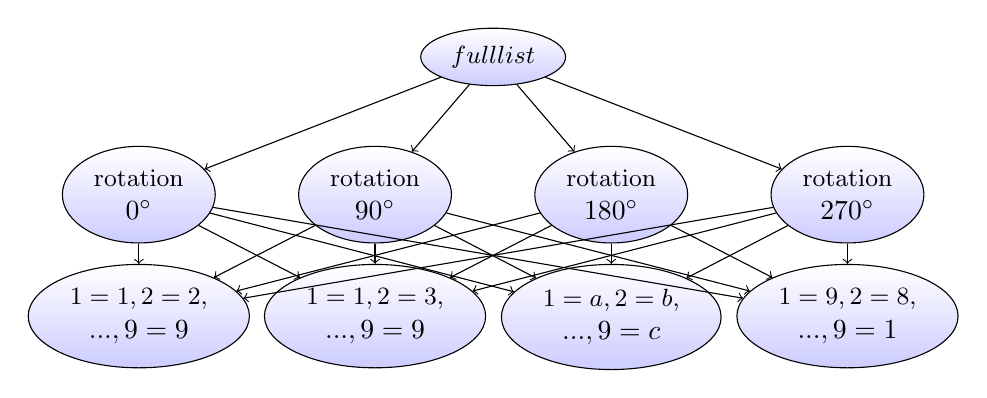
\begin{tikzpicture}[new set=import nodes, 
every node/.style = {ellipse, draw, align=center, anchor=north, 
                     top color=white, bottom color=blue!20}]]
\begin{scope}[nodes={set=import nodes}] % make all nodes part of this set
\node (full_list) at (3*1.5,4*1.5) {\small $full list$};
\node (0Rotation) at (0*1.5,3*1.5) {\small rotation \\ $0^\circ$};
\node (90Rotation) at (2*1.5,3*1.5) {\small rotation \\ $90^\circ$};
\node (180Rotation) at (4*1.5,3*1.5) {\small rotation \\ $180^\circ$};
\node (270Rotation) at (6*1.5,3*1.5) {\small rotation \\ $270^\circ$};
\node (1stNumberSwap) at (0*1.5,2*1.5) {\small $1=1, 2=2,$ \\ $...,  9=9$};
\node (2ndNumberSwap) at (2*1.5,2*1.5) {\small $1=1, 2=3,$ \\ $..., 9=9$};
\node (3rdNumberSwap) at (4*1.5,2*1.5) {\small $1=a, 2=b,$ \\ $..., 9=c$};
\node (4thNumberSwap) at (6*1.5,2*1.5) {\small $1=9, 2=8,$ \\ $..., 9=1$};
\end{scope}
\graph {
(import nodes);
% "import" the nodes
full_list -> {0Rotation, 90Rotation, 180Rotation, 270Rotation},
0Rotation -> {1stNumberSwap, 2ndNumberSwap, 3rdNumberSwap, 4thNumberSwap},
90Rotation -> {1stNumberSwap, 2ndNumberSwap, 3rdNumberSwap, 4thNumberSwap},
180Rotation -> {1stNumberSwap, 2ndNumberSwap, 3rdNumberSwap, 4thNumberSwap},
270Rotation -> {1stNumberSwap, 2ndNumberSwap, 3rdNumberSwap, 4thNumberSwap}
};
\end{tikzpicture}
\end{document}

\documentclass{book}
\usepackage{tikz}
\usetikzlibrary{graphs}

%\begin{document}
%\begin{tikzpicture}[new set=import nodes]
%\begin{scope}[nodes={set=import nodes}] % make all nodes part of this set
%\node [red] (a) at (0,1) {$a$};
%\node [red] (b) at (1,1) {$b$};
%\node [red] (d) at (2,1) {$d$};
%\end{scope}
%\graph {
%(import nodes);
%% "import" the nodes
%a -> b -> c -> d -> e;
%};
%\end{tikzpicture}
%\end{document}